\section{Appendix}
\label{sec:appendix}

\subsection{Benchmark details}

We present the evaluation benchmark sizes and the number of labels for each of the five benchmarks in \cref{tab:dataset}.

\begin{table}
\centering
\begin{tabular}{c|c|c}
    Benchmark & \# Samples & \# labels \\
    \hline
    ANLI & 1200 & 3 \\
    HANS & 30000 & 2 \\
    MNLI & 9815 & 3 \\
    SNLI & 9842 & 3 \\
    $\alpha$NLI & 1532 & 2 \\
\end{tabular}
\caption{Dataset details}
\label{tab:dataset}
\end{table}

\subsection{Prompt Templates}

The prompt templates used for each task are presented in \cref{tab:prompt_template}.

\begin{table*}[t]
    \centering
    \small
    \begin{tabular}{lp{8cm}}
        \toprule
        \textbf{Benchmark} & \textbf{Prompt Template} \\
        \midrule
        MNLI, SNLI, ANLI & \begin{verbatim}

Premise: {{ x["premise"] }}
Hypothesis: {{ x["hypothesis"] }}
A. Entailment
B. Neutral
C. Contradiction
Answer: {{ x["answer"] }}


Premise: {{ premise }}
Hypothesis: {{ hypothesis }}
A. Entailment
B. Neutral
C. Contradiction
Answer: {{ choice_text }}
\end{verbatim} \\
\midrule
AbductiveNLI & \begin{verbatim}

Observation 1: {{ x["obs1"] }}
Observation 2: {{ x["obs2"] }}
A. {{ x["choices"]["A"] }}
B. {{ x["choices"]["B"] }}
Answer: {{ x["answer"] }}


Observation 1: {{ obs1 }}
Observation 2: {{ obs2 }}
A. {{ choices["A"] }}
B. {{ choices["B"] }}
Answer: {{ choice_text }}
\end{verbatim} \\
\midrule
HansNLI & \begin{verbatim}

Premise: {{ x["premise"] }}.
Hypothesis: {{ x["hypothesis"] }}.
A. Entailment
B. Non-Entailment
Answer: {{ x["answer"] }}


Premise: {{ premise }}.
Hypothesis: {{ hypothesis }}.
A. Entailment
B. Non-Entailment
Answer: {{ choice_text }}
\end{verbatim} \\
\bottomrule
\end{tabular}
\caption{Prompt Templates for each task}
\label{tab:prompt_template}
\end{table*}

\subsection{Entropy vs Accuracy Plots}

\begin{figure*}[t]
    \centering
    \begin{subfigure}[b]{0.2\textwidth}
        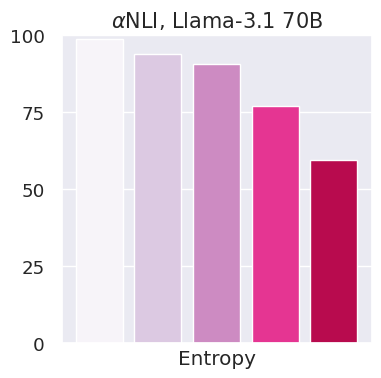
\includegraphics[height=2.6cm]{figures/appendix/entropy_acc_abductivenli_70B}
        \caption{}
    \end{subfigure}
    \begin{subfigure}[b]{0.2\textwidth}
        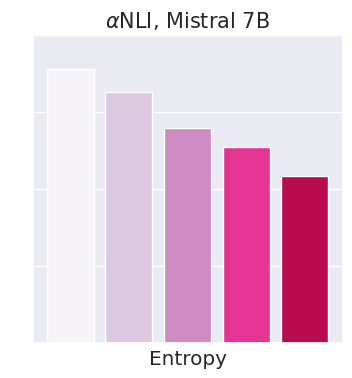
\includegraphics[height=2.6cm]{figures/appendix/entropy_acc_abductivenli_7B}
        \caption{}
    \end{subfigure}
    \begin{subfigure}[b]{0.2\textwidth}
        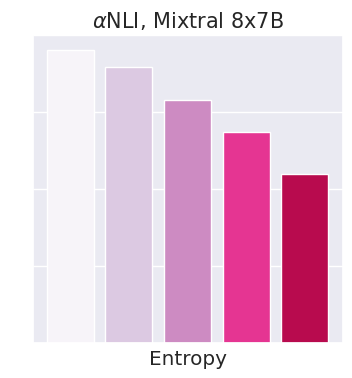
\includegraphics[height=2.6cm]{figures/appendix/entropy_acc_abductivenli_8x7B}
        \caption{}
    \end{subfigure}
    \begin{subfigure}[b]{0.2\textwidth}
        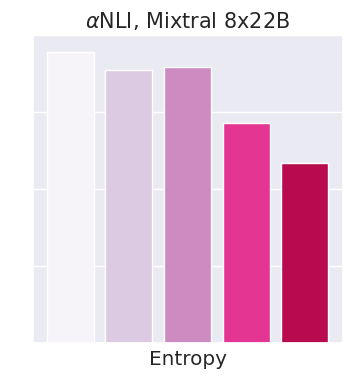
\includegraphics[height=2.6cm]{figures/appendix/entropy_acc_abductivenli_8x22B}
        \caption{}
    \end{subfigure}\\
    \begin{subfigure}[b]{0.2\textwidth}
        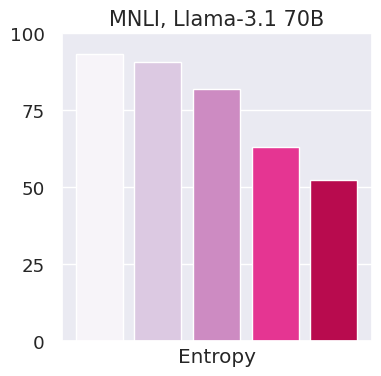
\includegraphics[height=2.6cm]{figures/appendix/entropy_acc_mnli_matched_70B}
        \caption{}
    \end{subfigure}
    \begin{subfigure}[b]{0.2\textwidth}
        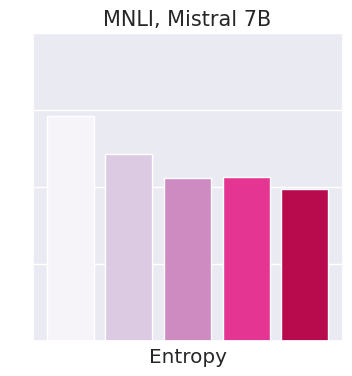
\includegraphics[height=2.6cm]{figures/appendix/entropy_acc_mnli_matched_7B}
        \caption{}
    \end{subfigure}
    \begin{subfigure}[b]{0.2\textwidth}
        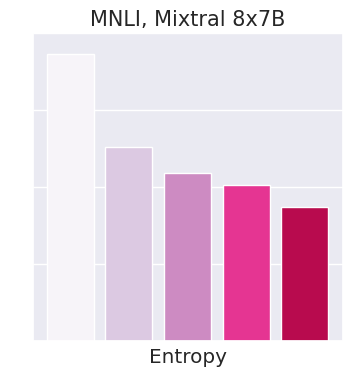
\includegraphics[height=2.6cm]{figures/appendix/entropy_acc_mnli_matched_8x7B}
        \caption{}
    \end{subfigure}
    \begin{subfigure}[b]{0.2\textwidth}
        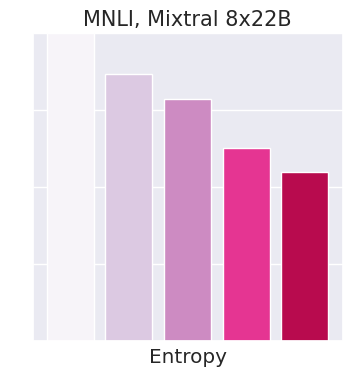
\includegraphics[height=2.6cm]{figures/appendix/entropy_acc_mnli_matched_8x22B}
        \caption{}
    \end{subfigure}\\
    \begin{subfigure}[b]{0.2\textwidth}
        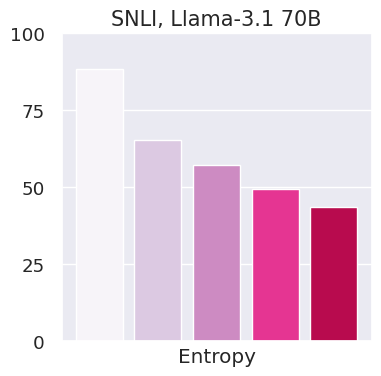
\includegraphics[height=2.6cm]{figures/appendix/entropy_acc_snli_70B}
        \caption{}
    \end{subfigure}
    \begin{subfigure}[b]{0.2\textwidth}
        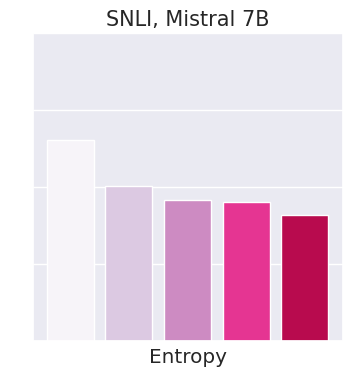
\includegraphics[height=2.6cm]{figures/appendix/entropy_acc_snli_7B}
        \caption{}
    \end{subfigure}
    \begin{subfigure}[b]{0.2\textwidth}
        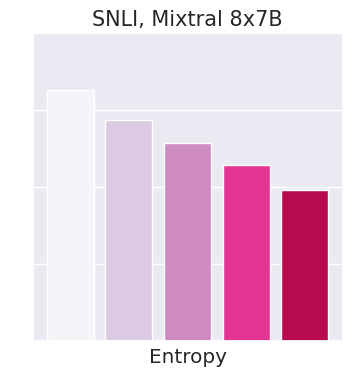
\includegraphics[height=2.6cm]{figures/appendix/entropy_acc_snli_8x7B}
        \caption{}
    \end{subfigure}
    \begin{subfigure}[b]{0.2\textwidth}
        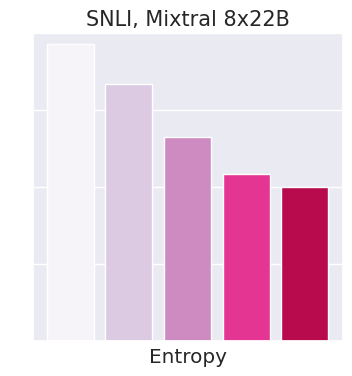
\includegraphics[height=2.6cm]{figures/appendix/entropy_acc_snli_8x22B}
        \caption{}
    \end{subfigure}
    \caption{\textbf{Accuracy versus entropy.} We show how the accuracy of all other models changes as the entropy of the human label distributions increases}
    \label{fig:entropy_accuracy_all}
\end{figure*}